\chapter{Introduction to succinct data structures}
\label{kap:kap1}

% TODOs: fixnut indexovanie, pridat viac prikladov pre succinct DS 

\section{Motivation}

In many applications, the amount of data is so significant that our choice of
the data structures we use is heavily influenced by their space usage. The field
of \textit{succinct data structures} focuses on representing data using as little
space as possible but at the same time tries not to hurt the time complexity and
performance of methods that these structures support. In this field, data structures for many
varied problems have been devised such as succinct dictionaries~\citep{raman2007succinct},
fenwick tree~\citep{bille2017succinct}, trie~\citep{grossi2015fast} or various text indexes.
While many of the resulting structures give some solid theoretical bounds on the used space,
others look into real-world space usage and performance.

Succinct data structures are very helpful in scenarios where we work with massive
amount of data. In these scenarios, using the ordinary data structures may limit us to place
the entire representation of data structure onto the slower type of memory storage. As succinct
data structures need to do the work of regular data structures but with additional constraints
on space used, they are often slower and more complicated than the alternatives using more
space. This is mainly because they do more work behind the scene and at the same time contain
concepts and computation patterns that are slow on modern computers. However, as we hinted
there are cases in which usage of space-efficient data structures speeds up the overall
running time as they enable us to store the data in a faster type of memory (e.g. fast RAM
instead of the slower disk). Thus, even if they use slower, more advanced concepts, the overall
runtime may decrease due to the lower amount of slow \textit{I/O operations}.

In this work, we are mainly concerned with \textit{bit vector}. One of the simplest
data structures that represents the sequence of zeroes and ones while supporting the
methods $\access$, $\rank$ and $\select$. Let us have a bit sequence $S$ and a bit
vector $B$ built on top of $S$. Using method $\access(i)$ over the $B$ simply returns
the $i$-th symbol in $S$. Method $\rank_c(i)$ returns the number of occurrences of
symbol $c$ in $S$ up to the $i$-th index. Method $\select_c(i)$ on the other hand
returns the index of $i$-th occurrence of symbol $c$ in $S$.

The reason behind our focus on bit vector and particularly its compressed version
is that it is one of the main building blocks of many succinct data structures.
In the next sections, we introduce some of its interesting and useful applications.

\section{Application 1: Sparse array}

Let $A$ be an array of $N$ elements each taking $k$ bits of space. We shall be interested in
accessing the $i$-th element of $A$. For simplicity, we assume that the elements of array may
not change after the construction. A straightforward representation of this array takes $N\cdot k$
bits of space. However, imagine a scenario where significant portion of the array is empty
and just a handful of elements are filled in. Take for example a sparse vector of numbers,
where most of the elements are 0. Then we could use a more space-efficient approach.
Let us assume that from $N$ elements only $n$ are non-default/non-zero and also that $n\ll N$.
First approach using the sparseness of an array is to store only the non-default elements as
pairs $(\text{position}, \text{value})$ where $\text{position}$ is an index where $\text{value}$
is located in $A$. This representation of pairs consumes $n\cdot (k+\log n)$ bits of space.
If we just store the pairs sorted by the position, accessing $i$-th element takes time $O(\log n)$.
We may use the hash table to obtain the constant time solution but this comes with additional
memory overhead. The alternative approach using the bit vector is to store non-default elements in
a packed array $P$ of length $n$ and size $nk$ bits. Alongside $P$ we store a bit vector $B$ of length
$N$ where
\[
   B[i]=
\begin{cases}
   1,& \text{if $A[i]$ is occupied} \\
   0,& \text{if $A[i]$ is empty/default value}
\end{cases}
\].

Using this representation of $A$, if we want to access $i$-th element in $A$, we first check for
the value of $B[i]$. If it is zero, we return the default value. If it is one, we need to find
how many ones are preceding this particular one in $B$ to locate where in array $P$ our non-default
value is placed. For this, we may use the $\rank_1$ method. Note, that method $\select_1$ can
be used to obtain the position of $i$-th non-default value in $A$. The total space used by this
representation is $N+n\cdot k+R$ where $R$ is the space needed to support an efficient $\rank$ query.
As we shall show in section~\ref{section:rank}, $\rank$ can be implemented in constant time with
sublinear space overhead, i.e., $R = o(N)$. If we are provided with bit vector implementation along
with $\access$ and $\rank$ methods we are able to reduce the total space used from $k\cdot N$ to
$N+n\cdot k+o(N)$ bits. Note that in practice, for really small number of non-default values, the
sparse array is still more interesting solution, however, bit vector provides us with a solution that
is often interesting in practice.

\section{Application 2: Storing elements of non-uniform length}

Let us consider another problem of representing an array of elements that are of variable length.
This type of elements can often arise in succinct data structures when trying to
optimise the amount of space used. An example of this is a \textit{Huffman code}
proposed by \cite{huffman1952method} that constructs the optimal code for symbols based
on the frequencies with which the symbols occur. This works in a way that more frequent
symbols are assigned bit code that is shorter while less frequent symbols get a longer code.
Even though we can store these elements one after another in memory, with the variable-length
elements, we do not have an easy and fast way to tell at which offset from the beginning of the
array the $i$-th is element located. Let us assume that we have $n$ elements of variable length.
First solution is to allocate the array of length $nk_{MAX}$ bits where $k_{MAX}$ is the number
of bits used for the element with the longest bit representation. This enables constant time access
but wastes a lot of space. The second possible solution is to allocate a bit array $R$ where
the elements are stored one after another in their raw bit representation. To locate the $i$-th element
we store alongside $R$ a helper array $P$. Number on $i$-th position is the index where the $i$-th
element begins in $R$. This helper array consumes at least $O(n\log n)$ bits as every entry
contains the number that is the index into the array $R$. This helper array can be replaced by bit vector.
The idea is to store the raw sequence of bits that store the elements one after another as in previous
solution. On top of that, we shall use a helper bit vector of the same size. This bit vector has ones on
places where the representation of some element starts and zeroes on all the other places. Example
of this representation can be seen in Fig.~\ref{obr:VariableSizedElements}.

Identifying the beginning of $i$-th element now boils down to efficiently locating the
$i$-th one in the helper bit vector. If we are provided with the bit vector implementation,
we can answer this using the $\select_1$ method. In chapter~\ref{kap:kap2}, we shall see how
this method can be implemented efficiently.

\begin{figure}
	\centerline{
	\begin{tabular}{l|l|l|l|l|l|l|l|l|l|l|}
	\cline{2-11}
	\textbf{Raw binary representation} & 1          & 1 & 0 & 1 & 1          & 1 & 1          & 0 & 1 & 0          \\ \cline{2-11} 
	\textbf{Beginning of an element}          & \textbf{1} & 0 & 0 & 0 & \textbf{1} & 0 & \textbf{1} & 0 & 0 & \textbf{1} \\ \cline{2-11} 
	\end{tabular}
	}
	\caption[TODO]{Raw binary representation of elements 1101, 11, 101 and 0 stored one after another.
	Note the helper bit array that is of the same size with ones on the positions where new element begins.}
	\label{obr:VariableSizedElements}
\end{figure}

\section{Application 3: FM-index}
% sources to help understand https://www.dcc.uchile.cl/TR/2005/TR_DCC-2005-004.pdf

For simplicity, in this section we assume that every text $T$ contains a special character
{\tt \$} located only at its end that is lexicographically smaller than any other character
contained in $T$.

Let us now consider another practically interesting problem. As we shall see, solution
to this problem also uses bit vector and other building blocks commonly used in succinct
data structures. This time, we have a text $T$ and are interested in \textit{indexing} it.
This means that if we get some pattern $P$, we would like to quickly answer questions such as
how many times is $P$ contained in $T$ and also where in $T$ these occurrences are located.
This is particularly useful in bioinformatics, where we can have a very long sequence of DNA and
are interested in searching for some subsequences in it. One of the solutions that is reasonably
fast and may be used is constructing \textit{suffix array} of $T$. Suffix array of $T$
is data structure that stores information about the lexicographical order of suffixes of $T$.

\begin{figure}
	\centerline{
        \begin{tabular}{l l l}
            i  & $S$ & suffix\\
        \hline
            \small 0& 7	& \tt \$ \\
            \small 1& 6 & \tt a\$ \\
            \small 2& 4 & \tt ana\$ \\
            \small 3& 2 & \tt anana\$ \\
            \small 4& 1 & \tt banana\$ \\
            \small 5& 5 & \tt na\$ \\
            \small 6& 3 & \tt nana\$ \\
        \end{tabular}
	}
	\caption[TODO]{
        Suffix array $S$ of $T = \mathtt{banana\$}$
    }
	\label{obr:suffixArray}
\end{figure}

More precisely, on $i$-th position of suffix array $S$, it stores the starting position of
suffix that comes $i$-th in lexicographical order. The example of suffix array is in
Fig.~\ref{obr:suffixArray}. Searching for pattern $P$ in suffix array of $T$ uses fact that
if $P$ is contained in $T$ it will be at the beginning of some suffixes that make up a
continuous subsequence of $S$. Succinct data structure that is in some aspects similar to
suffix array was proposed by \cite{ferragina2000opportunistic} and is called \textit{FM-index}.
FM-index can find the pattern in the preprocessed text in time complexity $\BigO(|P|)$. On top
of this, the resulting space used by FM-index can be even smaller than the space used for the original
text $T$. This makes FM-index particularly useful for searching in very long DNA sequences where
FM-index many times takes just 30-40\% of the space needed for the representation of original text
$T$ as was observed by \cite{ferragina2001experimental}. We shall now look at how the FM-index
is obtained for the text $T$.

\paragraph{Burrows-Wheeler transformation}

\textit{Burrows-Wheeler transformation~(BWT)} proposed by \cite{burrows1994block} is a pivotal
part of the FM-index. BWT of a text $T$ gives us a sequence $\mathit{T_{BWT}}$ of the same
length. Furthermore, this operation is reversible in a sense that only using $\mathit{T_{BWT}}$
we are able to reconstruct the original text $T$. This transformation is used as a
preprocessing step of some compression algorithms such as \textit{bzip2} introduced by
\cite{seward1996bzip2} and was studied more by \cite{manzini2001analysis}. This is because
BWT is oftentimes easier to compress. We shall show how it is constructed and then give 
intuition why it has this property. We consider the sequence $T$ of symbols over some
alphabet $\Sigma$. Now we take all the cyclical rotations $T_1, T_2, \ldots T_n$ of
the sequence $T$ and imagine putting them sorted by their lexicographical order into the
rows of table $M$ as seen in Fig.~\ref{obr:BWT}. We name the sequence created by the
concatenation of symbols in first and last column $F$ and $L$ respectively. Last column $L$
is what we call the BWT of $T$. Note that the sequence $F$ can be obtained from $L$ just by
sorting all the characters in $\mathit{T_{BWT}}$ and has also some useful properties. $F$ consists
of runs of symbols that are sorted according to the lexicographical ordering of alphabet symbols.
We shall use the helper sequence $\Count$ where $\Count[c]$ is number of occurrences of symbols
smaller than $c$. Note that the run of symbol $c$ in $F$ starts at the index $\Count[c]+1$. The
matrix $M$ contains all the suffixes sorted according to their lexicographical order.

\begin{figure}
	\centerline{
	\begin{tabular}{l|c|ccccc|c|}
	\cline{2-8}
	  & $F$ & \multicolumn{5}{l|}{} & $L$   \\ \cline{2-8} 
	1 & {\tt \$}	& \multicolumn{1}{c|}{{\color[HTML]{C0C0C0} \tt b}}		& \multicolumn{1}{c|}{{\color[HTML]{C0C0C0} \tt a}}	& \multicolumn{1}{c|}{{\color[HTML]{C0C0C0} \tt n}}	& \multicolumn{1}{c|}{{\color[HTML]{C0C0C0} \tt a}}	& {\color[HTML]{C0C0C0} \tt n}  & {\tt a}  \\ \cline{2-8} 
	2 & {\tt a}  		& \multicolumn{1}{c|}{{\color[HTML]{C0C0C0} \tt \$}} 	& \multicolumn{1}{c|}{{\color[HTML]{C0C0C0} \tt b}}	& \multicolumn{1}{c|}{{\color[HTML]{C0C0C0} \tt a}}	& \multicolumn{1}{c|}{{\color[HTML]{C0C0C0} \tt n}}	& {\color[HTML]{C0C0C0} \tt a}  & {\tt n}  \\ \cline{2-8} 
	3 & {\tt a}		& \multicolumn{1}{c|}{{\color[HTML]{C0C0C0} \tt n}}		& \multicolumn{1}{c|}{{\color[HTML]{C0C0C0} \tt a}}	& \multicolumn{1}{c|}{{\color[HTML]{C0C0C0} \tt \$}}& \multicolumn{1}{c|}{{\color[HTML]{C0C0C0} \tt b}}	& {\color[HTML]{C0C0C0} \tt a}	& {\tt n}  \\ \cline{2-8} 
	4 & {\tt a}		& \multicolumn{1}{c|}{{\color[HTML]{C0C0C0} \tt n}}		& \multicolumn{1}{c|}{{\color[HTML]{C0C0C0} \tt a}}	& \multicolumn{1}{c|}{{\color[HTML]{C0C0C0} \tt n}}	& \multicolumn{1}{c|}{{\color[HTML]{C0C0C0} \tt a}}	& {\color[HTML]{C0C0C0} \tt \$}	& {\tt b}  \\ \cline{2-8} 
	5 & {\tt b}		& \multicolumn{1}{c|}{{\color[HTML]{C0C0C0} \tt a}}		& \multicolumn{1}{c|}{{\color[HTML]{C0C0C0} \tt n}}	& \multicolumn{1}{c|}{{\color[HTML]{C0C0C0} \tt a}}	& \multicolumn{1}{c|}{{\color[HTML]{C0C0C0} \tt n}}	& {\color[HTML]{C0C0C0} \tt a}  & {\tt \$} \\ \cline{2-8} 
	6 & {\tt n}		& \multicolumn{1}{c|}{{\color[HTML]{C0C0C0} \tt a}}		& \multicolumn{1}{c|}{{\color[HTML]{C0C0C0} \tt \$}}& \multicolumn{1}{c|}{{\color[HTML]{C0C0C0} \tt b}}	& \multicolumn{1}{c|}{{\color[HTML]{C0C0C0} \tt a}}	& {\color[HTML]{C0C0C0} \tt n}  & {\tt a}  \\ \cline{2-8} 
	7 & {\tt n}		& \multicolumn{1}{c|}{{\color[HTML]{C0C0C0} \tt a}}		& \multicolumn{1}{c|}{{\color[HTML]{C0C0C0} \tt n}}	& \multicolumn{1}{c|}{{\color[HTML]{C0C0C0} \tt a}}	& \multicolumn{1}{c|}{{\color[HTML]{C0C0C0} \tt \$}}& {\color[HTML]{C0C0C0} \tt b}  & {\tt a}  \\ \cline{2-8} 
	\end{tabular}
	\hspace{4em}
	\begin{tabular}{l l l}
		sorted suffixes\\
	\hline
		\tt \$ \\
		\tt a\$ \\
		\tt ana\$ \\
		\tt anana\$ \\
		\tt banana\$ \\
		\tt na\$ \\
		\tt nana\$ \\
	\end{tabular}
	}
	\caption[TODO]{On the left we can see the matrix $M$ filled with cyclic rotations of sequence
	$S = \mathtt{banana\$}$. On the right, we can see the sorted suffixes (content of suffix array). The
	Burrows-Wheeler transformation of $S$ is string $L=\mathtt{annb\$aa}$ -- the last column of $M$.
	Note that in practice, we do not need to construct the whole table as more efficient algorithms exist.
	It is also notable that matrix $M$ includes very similar information to suffix array.
	}
	\label{obr:BWT}
\end{figure}

The reason that BWT is more compressible is that it frequently contains runs of the same
symbol. This can be better explained on an example. Let us create BWT of a text containing
a lot of mentions of word {\tt computer}. All the rotations prefixed with {\tt omputer} will form a
continuous subsequence of rows of $M$. If we assume, that word {\tt computer} is very frequent
in the text, most of these rows will contain {\tt c} at the end as this is the most common symbol
preceding word {\tt omputer}. This will for example create the common run of symbol {\tt c} in BWT.

\paragraph{Searching in an FM-index}

As we already stated, FM-index is used for searching in the preprocessed text.
Searching in FM-index is based on the two important properties:

\begin{enumerate}
	\item Suffixes containing word $w$ as a prefix form a consecutive subsequence of rows in $M$.
	\label{chapter1:fmindexprop:prop1}
	\item The $i$-th occurence of character $c$ in $F$ corresponds to the $i$-th occurence of $c$ in $L$.
	\label{chapter1:fmindexprop:prop2}
\end{enumerate}

First property was also what enabled us to search for a pattern in a suffix array.
The second property is less trivial to observe. Let us take two rows in $M$, $T_i$ and $T_j$
such that $i<j$. Let $T_i$ be of the form $cxA$ and $T_j$ of the form $cyB$ where $c, y$ are
characters of the text and $A$ and $B$ are sequences of characters. As $i<j$ it follows that
either $x<y$ or $x=y$ and $A<B$ but this also means that after rotating these two rows we get
sequences $xAc$ and $yBc$ respectively. It can be observed that $xAc$ will also preceed $yBc$
in this case. From this observation, it follows that the relative ordering of the same character
is maintained from $F$ to $L$.

The search for rows where pattern $P$ is located will proceed from the end of $P$. This works by
finding rows where suffixes $P[n\ldots], P[n-1\ldots]$ etc. are located. At every step, these
rows will form a continuous subsequence of rows of $M$ so we will store only its beginning and end.
This follows from the observation \ref{chapter1:fmindexprop:prop1}. Let us assume that we are
looking for a word {\tt house} and we already found the range of rows in $M$ that have {\tt ouse}
as their prefix. If we look to the last column, these symbols correspond to the symbols preceding
{\tt ouse} in the text. We can maybe see there in arbitrary order symbols like {\tt m} for word
{\tt mouse} or {\tt h} for {\tt house}. To search for the range of rows in $M$ that have as a prefix
word ({\tt house}) we shall look into the range of all prefixes beginning with {\tt h}. Locating this
range is easy thanks to the $\Count$ helper array. Lines in this range are sorted according to the
second character so there will be some lines continuing with {\tt a} if the text contained for example
word {\tt hashtag} or {\tt e} if the word {\tt head} was in the text. Somewhere the lines starting with 
{\tt house} will be located, but we do not store anything except for $T_{BWT}$ and $\Count$.
However, we already located the range where suffixes starting with {\tt ouse} are located in.
We can look how many times {\tt h} is located before this range in $T_{BWT}$. Thanks to this
number and the property \ref{chapter1:fmindexprop:prop2}, we know where in $F$ the subsequence
containing the prefix {\tt house} begins.

% TODO: mozno obrazok

The process will in general proceed in these steps:

\begin{itemize}
	\item We find where $P[n-1]$ is located in $M$. This means setting beginning~($b_{n-1}$) and
	the end~($e_{n-1}$) of the current subsequence to $\Count[P[n-1]]+1$ and $\Count[P[n-1]+1]$
	respectively.
	\item Now, to found where $P[n-2..]$ is located in $M$, we would like to locate occurrences
	of $P[n-1]$ that are preceded by $P[n-2]$. In other words, would like to find all
	occurrences of symbol $P[n-2]$ in $L[b_{n-1}..e_{n-1}]$. However, this is not trivial
	as they can be at arbitrary places in this subsequence, even not in a continuous
	subsequence. Instead of searching in $L$ we look at the occurrences of symbol $P[n-2]$ in
	$F$. Here, they are sorted and it is easy to tell, which of these are followed by
	$P[n-1]$ as $i$-th occurence of character $P[n-1]$ in $L$ corresponds to $i$-th
	occurence of $P[n-1]$ in $F$. Using this fact, we set
	$b_{n-2} = \Count[P[n-2]] + \rank_{P[n-2]}(b_{n-1})$ and
	$e_{n-2} = \Count[P[n-2]] + \rank_{P[n-2]}(e_{n-1})$. Here $\Count[P[n-2]]$
	is the index where run of character $P[n-2]$ starts. $\rank_{P[n-2]}(b_{n-1})$
	is number that gives us number of occurrences of character $Count[P[n-2]]$ in $L$ that
	preceded the index $b_{n-1}$ (starting index of the previous subsequence).
	\item We continue and repeat this process until we compute $b_1$ and $e_1$ or until
	$b_i=e_i$.
\end{itemize}

As we can see, we are not only interested in $\rank$ over a bit vector but also over an arbitrary
alphabet that we would like to use in the FM-index. This seems like an even harder task.
In the next section, we shall see how we can reduce this problem and use the bit vector
implementation also for the $\rank$ and $\select$ over the general alphabet.

\paragraph{Wavelet tree}
\label{section:WaweletTree}

We shall assume for a moment that we have a bit vector implementation supporting
$\access$, $\rank$ and $\select$ methods. We show how this may be used to create
a more general version of this implementation representing sequence over arbitrary
alphabet still supporting $\access$, $\rank$ and $\select$ queries in reasonable time complexity.

The most straightforward approach is to store one bit vector of size $|S|$,
per every character of the alphabet $\Sigma$. Let us call these bit vectors $B_1,
B_2, \ldots B_{\sigma}$. Each of them stores ones on positions where the symbol corresponding
to this bit vector is located, according to the formula

\[
    B_i[j]= 
\begin{cases}
	1,& \text{if } S[j]=i \\
    0,& \text{otherwise}
\end{cases}
\].

This is indeed very fast because we support $\rank$ and $\select$ in the exact same time
that our bit vector implementation of $\rank$ and $\select$ is running in. However, we use
roughly $|\Sigma|$ times more space.

\textit{Wavelet tree} uses a divide-and-conquer approach. It takes the sequence $S$ of
length $n$ over some alphabet $\Sigma$ and recursively splits the alphabet into
two subsets creating a hierarchical partitioning of an alphabet. In the root node
of the tree, it splits the alphabet $\Sigma$ into two subsets $\Sigma_1$ and $\Sigma_2$
of roughly equal size. It then stores a bit vector $B$ of size $n$ in this node
where
\[
    B[i]= 
\begin{cases}
    0,& \text{if } S[i]\in \Sigma_1\\
    1,              & \text{otherwise}
\end{cases}
\]

Then it creates two strings $S_1$ and $S_2$ from $S$ by taking just symbols
from $\Sigma_1$ and $\Sigma_2$ respectively. The left and right children of the root node
are then built by recursively applying the same idea on the subsequences $S_1$ and $S_2$.

\begin{figure}
	\centerline{
		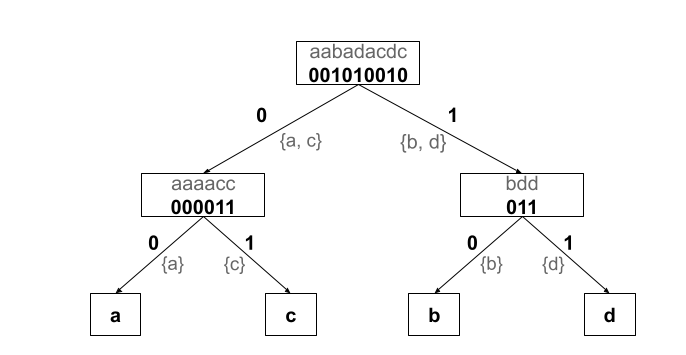
\includegraphics[width=0.9\textwidth, height=0.3\textheight]{images/wavelet_tree}
	}
	\caption[TODO]{Wavelet tree representation of text $S=\mathit{aabadacdc}$. We can see how
	the recursive partitioning of the alphabet works. In every node, we also show the
	subsequence represented (grey text) in the subtree of the node. The stored data can be
	recognized as they are in bold and black.
	}
	\label{obr:WaveletTreeExample}
	% based on https://simongog.github.io/assets/data/sdsl-slides/tutorial#23
	% source at https://docs.google.com/drawings/d/1cJyda3bdTluajr3iXu1x1iL5HF0JPZqAHw6jwct9KLI/edit
\end{figure}

Both $\rank$ and $\select$ methods on the original sequence can be implemented using the tree
traversal and $\rank$/$\select$ methods on the individual bit vectors. Another modification
studied by \cite{makinen2005succinct} is to shape the binary tree in a way that a Huffman
tree of the sequence symbols is shaped. Huffman tree is a tree constructed in the
process of creating Huffman encoding of the characters contained in the sequence.

\section{Space efficiency}

There are many ways to measure the space efficiency of a data structure. From the
practical point of view, we may be interested in the memory usage by the data
structure on actual data that the structure could encounter in our use case. However,
many succinct data structures are trying to achieve some upper bounds and express
the used space in terms of the information contained in the data. There are many
models how to measure the information contained in sequences of characters. One
of the most commonly used models in the field of succinct data structures, yet still
quite simple, is entropy or more specifically zeroth-order entropy:

$$H(S)=\sum_{c\in\Sigma} \frac{n_c}{n} \lg \frac{n}{n_c}$$.

In many scenarios, where succinct data structures are used, the stored sequence
is compressible using the sole fact that some symbols have a bigger frequency than others.